\let\negmedspace\undefined
\let\negthickspace\undefined
\documentclass[journal]{IEEEtran}
\usepackage[a5paper, margin=10mm, onecolumn]{geometry}
\usepackage{tfrupee}

\setlength{\headheight}{1cm} 
\setlength{\headsep}{0mm}     

\usepackage{gvv-book}
\usepackage{gvv}
\usepackage{cite}
\usepackage{amsmath,amssymb,amsfonts,amsthm}
\usepackage{algorithmic}
\usepackage{graphicx}
\usepackage{textcomp}
\usepackage{xcolor}
\usepackage{txfonts}
\usepackage{listings}
\usepackage{enumitem}
\usepackage{mathtools}
\usepackage{gensymb}
\usepackage{comment}
\usepackage[breaklinks=true]{hyperref}
\usepackage{tkz-euclide} 
\usepackage{array}                                            
\usepackage{longtable}                                       
\usepackage{multirow}                                         

\begin{document}

\bibliographystyle{IEEEtran}
\vspace{3cm}

\title{2.10.76}
\author{EE25BTECH11048 - Revanth Siva Kumar.D}
{\let\newpage\relax\maketitle}
\textbf{Question}
Find the equation of the line joining the points $(3,1)$ and $(9,3)$. 

\textbf{Solution :} 

Given 
\begin{align}
    \vec{A}=\myvec{3\\1} \vec{B}=\myvec{9\\3} 
    \label{eq:points}
\end{align}
Let us assume line equation to be:
\begin{align}
    \vec{n}^T \vec{x} = c
\end{align} 
    We get the line equation on solving \[\myvec{\vec{A}&\vec{B}}^T\vec{n}=c\myvec{1\\1}\] 

The line passes through the points from \eqref{eq:points} substituting, we get:
\begin{align}
    \myvec{3 & 9 \\
       1 & 3  }^T\vec{n}=c\myvec{1 \\ 1}
\end{align}

\begin{align}
    \myvec{3 & 1 \\
       9 & 3  }\vec{n}=c\myvec{1 \\ 1}
\end{align}
Now by Gaussian Elimination solve:
\begin{align}
\myvec{3 & 1 & \big| & 1 \\
         9 & 3 & \big| & 1 }
\end{align}

\begin{align}
R_{1} &\leftarrow \frac{1}{3}R_{1} \nonumber\\
\Rightarrow\ 
&\myvec{1 & \frac{1}{3} & \big| & \frac{1}{3} \\
         9 & 3 & \big| & 1 }
\end{align}

\begin{align}
R_{2} &\leftarrow R_{2}-9R_{1} \nonumber\\
\Rightarrow\ 
&\myvec{1 & \frac{1}{3} & \big| & \frac{1}{3} \\
         0 & 0 & \big| & -2 }
\end{align}
By the assumption that line equation is $\vec{n}^T\vec{x}=1$ which doesn't pass through origin we are not getting any solution.So our assumption is wrong and origin lies on the line . 
So consider \begin{align}
    \vec{n}^T \vec{x} = 0
\end{align} 
$c=0$ because origin lies on the line and solving:
so now,Assume the line equation:
\[
\vec{n}^T \vec{x} = 0, \quad 
\vec{n} = \myvec{n_1\\n_2}
\]

 

Line passes through points $\vec{A}$ and $\vec{B}$

\begin{align}
\vec{n}^T \vec{A} = 0 \implies 3 n_1 + 1 n_2 = 0
\end{align}
\begin{align}
    \vec{n}^T \vec{B} = 0 \implies 9 n_1 + 3 n_2 = 0
\end{align}


Matrix form:
\begin{align}
    \myvec{3 & 1 \\ 9 & 3} \myvec{n_1\\n_2} = \myvec{0\\0}
\end{align}

Augmented matrix:
\begin{align}
\myvec{3 & 1 &\big|& 0 \\ 9 & 3 & \big| & 0}
\end{align}
\begin{align}R_{1} &\leftarrow \frac{1}{3}R_{1} \nonumber\\&
\Rightarrow \myvec{1 & \frac{1}{3} & \big| & 0 \\ 9 & 3 & \big| & 0}
\end{align}

\begin{align}R_{2} &\leftarrow R_{2}-9R_{1} \nonumber\\&
\Rightarrow \myvec{1 & \frac{1}{3} & \big| & 0 \\ 0 & 0 & \big| & 0}
\end{align}

From first row:
\begin{align}
n_1 + \frac{1}{3} n_2 = 0 \implies n_1 = -\frac{1}{3} n_2\\
\end{align}
Let,
\begin{align}
n_2 = 3 \implies n_1 = -1\\
\vec{n} = \myvec{-1\\3}
\end{align}

\begin{align}
    \vec{n}^T \vec{x} = 0 \implies \myvec{-1 & 3} \vec{x} = 0 
\end{align}
The equation of the line passing through $(3,1)$ and $(9,3)$ is:
\[\boxed{\myvec{-1 & 3} \vec{x} = 0 }\]
\begin{figure}[H]
    \centering
    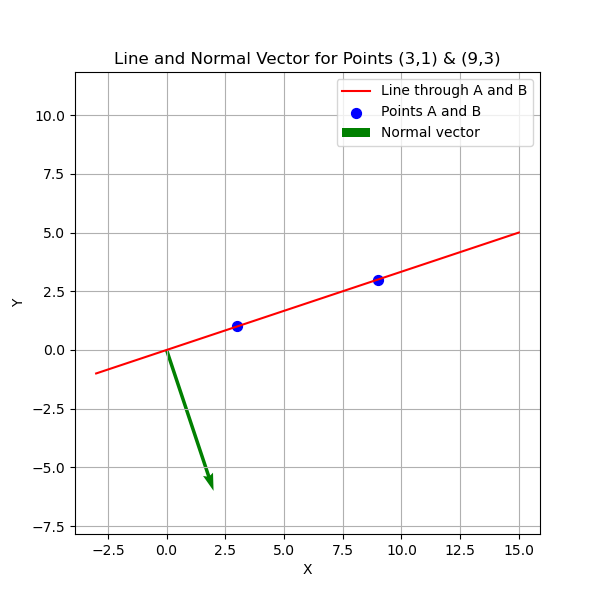
\includegraphics[width=0.8\columnwidth]{figs/Figure_1.png}
    \caption{PLOT}
    \label{fig:fig1}
\end{figure}
\end{document}
